%!TEX program = xelatex
\documentclass[a4paper]{ctexart}
\usepackage{CJK}
\usepackage{graphicx}
\usepackage{float}
\usepackage{subfigure}
\usepackage{hyperref}
\usepackage{longtable}

% Title Page
\title{光电心率计}
\author{指导教师:吴裕斌 \\ 班级:光电2004班\\姓名:姚海舟\\学号:U202014528\\同组者:汪鑫书 \ 李博函\\联系电话:13720213247}

\begin{document}
\maketitle
\thanks{Solution chosen by Timicasto Index}
\newpage
\tableofcontents

\newpage
\begin{abstract}
	基于光电容积描记术(PPG)的光学心率检测系统,该系统由发射器控制模块,接收器模块,带通滤波模块和信号分析模块组成,脉搏信号依次通过上述模块处理后得到最终精确的脉搏。
\end{abstract}


\newpage
\section{技术指标}

	实时信号预处理,在每个脉搏产生后立刻可见心室收缩间隔时间,可用于监测心率不齐等,可处理30~260bpm间的脉搏数据
	
	带有谐波的 700kHz/1Ksps 波形显示与记录
	
	一体化透明盖板,带有为提高光效率和采样精度设计的聚光透镜和变向棱镜二合一的外形

\newpage
\section{基本原理}

	本系统使用PPG (光电容积描记术) 完成脉搏信号量测,将光照射进皮肤,当血流动力发生变化时,就会可预见地散射光。
	
	氧合血红蛋白在可见光范围内有550nm和600nm两个吸收峰,使用绿光LED将光射入皮肤,则光电二极管上流过的电流曲线即为血流动力的变化曲线。
	
	反射光强达最大值时即为此处皮肤中动脉搏动即心室收缩的时刻,因为心率的定义为两次心室收缩的时间间隔,所以记录相邻的两次时刻并计算其间隔即为此刻的心率

\newpage
\section{方案论证}
	
	PPG有两个关键的核心过程,就是信号的发射与采集,氧合血红蛋白的吸收光谱在400nm呈现出最高的一个峰,在550和600nm上有次高的两个峰。
	
	因为只有在吸收峰上的光才会是被血红蛋白正确吸收,而400nm的LED灯又太过昏暗,于是这里选用了主波长为540~560nm的LED灯作为发射源。
	
	而光电二极管是可以把特定范围波长的光强转化为电流信号的器件,此处选择可以响应540~560nm波长的光电二极管即可最好地接收反射的光信号.
	
	然而这里接受到的信号是比较微弱的电流信号,还需要使用跨阻放大器将其转换为电压信号,并使用增益可变的放大器将电压信号放大,来适应不同的皮肤透射率,不同环境光强,皮肤与传感器不同距离的使用场景。
	
	放大得到的信号还含有皮肤等其它组织反射的恒定光,表现为直流分量,和大量的被测皮肤运动产生的高频噪声,此处使用带通滤波器将其滤除后将信号送入STM32的12位ADC。
	
	由于此系统需要处理最大达260bpm即4.3Hz的信号,则为了更好地还原波形和更好的数据实时性,将ADC配置为12bit精度和1Ksps的采样率,分别采样10Hz以上被滤除的信号和4.3Hz以上被滤除的信号,用于波形显示和心率计算。
	
	\cite{Activity:HRM Circuit}
	\cite{HRM Circuit}

\newpage
\section{硬件电路设计}

	对于主控MCU的选型,考虑到此系统的运算量不大,在成本和功耗的考虑下选择了STM32G0x0低成本系列MCU,得益于G0系列不需要晶振的特点,也可以节省板上空间,而此系统中共需要调试接口,屏幕,可变增益放大器,采集到的心率信号,LED控制共五组IO,则选择具有20引脚,成本最低的的FxP封装。
	
	由于所有的IO全部都是常用嵌入式接口或GPIO,则选用G0x0中最低端的型号G030F6P作为此系统的主控。
	
	MCU的供电部分,使用具有3x3 QFN小封装低成本的TLV62130构造了2.5MHz的高效率开关电源输出系统3.3V供电,变换器的效率可达0.89,且仅占用了3x5mm的板面积,可输出最大3A的电流。
	
	用户界面使用了一块1.44in,具有128x128分辨率,262K色的普通TFT-LCD屏幕和 $50cd/m^2$的WLED背光,配合ST7735S控制芯片,使用五个IO接口,分别传输显示数据,显示时钟,重置信号,命令/数据标志信号和背光信号。
	
	经过对分销商平台上所有LED的筛选,最终选择了两颗来自Vishay的 VLMTG41S2U1-GS08 ,这颗LED使用InGaN技术部分攻克了绿光LED的亮度难题,在3.2V的正向电压下达到了至少560mcd的亮度,且波长偏离不超过+-15nm。
	
	光电二极管的选型遇到了一点难题,绝大多数光电二极管是设计用来接收红外遥控信号的,所以完全不会响应可见光。
	
	经历了海量的搜索后,仍然是在Vishay找到了我们想要的东西:VEMD5510C,它的响应峰值波长刚好为550nm,只响应440~700nm之间的光,完全符合本系统的波长需要。
	
	因为VEMD5510C只有0.2mm厚,而我们的LED却是标准的3528封装,有1.75mm厚,于是我们把光电二极管夹在了两颗LED之间,并在上面加上了一体式的聚光和变向棱镜。
	
	放大器的部分,因为心率信号的带宽很低,所以为成本考虑选择了双路LM2904运算放大器,并使用TPS60403电荷泵作为负压源,使用三颗LM2904构造起了跨阻放大器,可变增益放大器和后级的带通滤波器。
	
	VEMD5510C在1000 lx下有10uA的电流,于是我们采用了增益为5dB的跨阻放大器,将0~10uA的信号转换至0~2.5V,让可变增益放大器具有更大的操作空间。
	
	在设计可变增益放大器时再次遇到了难点。
	
	市面上的PGA芯片都达到了动辄百元的高价,并且增益配置也不够自由,于是我们想到了使用数字电位器作为普通正增益运算放大器的反馈电阻,本来以为数字电位器不是设计用于做这样的事情的,结果意外地真的找到了可以用于这种用途的数字电位器:使用I2C协议的AD5272。
	
	于是PGA的设计顺理成章,使用AD5272BCPZ-20设计了0~20倍放大倍数可变的放大器。
	
	最后一个难题就是滤波器了。
	
	本系统中的有效信号频率介于0.4~4.3Hz之间,我们选用了增益曲线较平缓的二级Butterworth滤波器作为高通滤波器,滤除0.4Hz以下的信号,但是这里第二级反馈系统的电容太大了,数值也太离谱了。
	
	先是到了离谱的80uF,调低了阻断频带衰减率后变成了20.5uF和16uF,取E6系列电容的近似值则为33uF和15uF,勉勉强强找到了尺寸为0805的MLCC电容,免除了使用大号电解电容的麻烦。
	
	然后用阻断频带为10Hz和4.3Hz的低通滤波器,分别输出用于波形显示和用于心率计算的信号给STM32的ADC1 CH0和CH1。

	整个PCB的板框尺寸与屏幕的尺寸一致,使用四个M2螺丝和屏幕固定为一体,其它所有电阻电容均选用0603封装的型号。
	
	至此完成了上面的电路原理设计和布局布线后,硬件的设计就全部完成了

\newpage
\section{软件设计}

	软件部分使用现代C/C++语言(C23/C++23),引入STM32 HAL库与硬件交互,并完全符合现代OOP编程范式。
	
	所有硬件初始化代码使用STM32CubeMX生成,构建系统文件基于STM32CubeMX生成的Makefile修改,使其支持C++的编译和链接。
	
	数据采集部分,我们初始化了一个每秒溢出1000次的Timer,用TRGO事件触发ADC的采集,每完成一次采集触发中断后开始处理数据,将电压幅值数据送入心率算法对象。
	
	心率算法类接受电压幅值作为输入,使用一次心率周期进行电压范围校准后,钳制在校准数据峰值三分之二以上的部分为有效峰值数据区域,同时维护当前周期最大幅值和其对应的绝对采样次数,当下一次幅值进入有效峰值窗口时将当前数据记录为上一周期 与当前周期作差后计算时间间隔对应的心率。
	
	当两个周期的数据均有效,并成功计算出心率后,在主循环中将其发送至屏幕显示。

\newpage
\section{测试报告}

\begin{figure}[H]
	\centering
	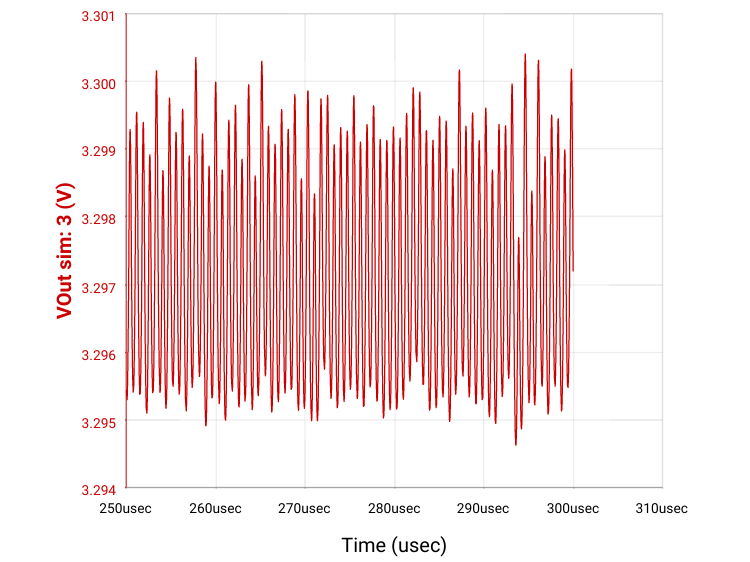
\includegraphics[width=1.0\textwidth]{amCharts.png}
	\caption{电源纹波测试:5.78mV Peak-to-Peak}
\end{figure}

\begin{figure}[H]
	\centering
	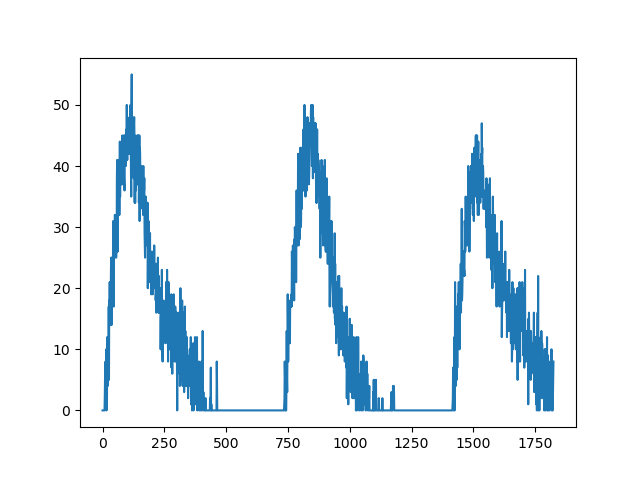
\includegraphics[width=1.0\textwidth]{ppg.png}
	\caption{原始电平波形,Y轴单位长度0.8mV}
\end{figure}	


\newpage
\section{结论}
	
	本课程设计报告详细阐述了一个基于光电容积描记术(PPG)的光学心率检测系统的设计和实现。系统由发射器控制模块,接收器模块,带通滤波模块和信号分析模块组成,能够实时处理和显示30~260bpm间的脉搏数据。
	
	在硬件和软件设计部分,我们选择了STM32G0x0低成本系列MCU作为主控,使用了现代C/C++语言(C23/C++23),引入STM32 HAL库与硬件交互。测试结果显示,该系统能够准确地测量和显示心率数据.

\section{免责声明}
	\textbf{此设计不可用于生命攸关的医疗设备,除非已由双方授权官员签署了专门管控此类使用情况的特殊合同}
	
	\textbf{使用风险自负}
	
	\textbf{This design may not used in life-critical medical equipment unless authorized officers of the parties have executed a special contract specifically governing such use.}
	
	\textbf{USE AT YOUR OWN RISK.}

\newpage
\begin{thebibliography}{20}
	\bibitem{Activity:HRM Circuit}\href{https://wiki.analog.com/university/courses/alm1k/alm-lab-heart-rate-mon}{Doug Mercer. Activity: Heart Rate Monitor Circuit[R].Analog Wiki, 14 May 2022}
	\bibitem{HRM Circuit}\href{https://www.homemade-circuits.com/heart-rate-monitor-alarm-circuit/}{Swagatam. Heart Rate Monitor Circuit[J]. Homemade Circuit Projects, October 18, 2019}
\end{thebibliography}

\end{document}          
